\documentclass[a4paper]{article}
\usepackage[]{graphicx}\usepackage[]{color}
% maxwidth is the original width if it is less than linewidth
% otherwise use linewidth (to make sure the graphics do not exceed the margin)
\makeatletter
\def\maxwidth{ %
  \ifdim\Gin@nat@width>\linewidth
    \linewidth
  \else
    \Gin@nat@width
  \fi
}
\makeatother

\definecolor{fgcolor}{rgb}{0.345, 0.345, 0.345}
\newcommand{\hlnum}[1]{\textcolor[rgb]{0.686,0.059,0.569}{#1}}%
\newcommand{\hlstr}[1]{\textcolor[rgb]{0.192,0.494,0.8}{#1}}%
\newcommand{\hlcom}[1]{\textcolor[rgb]{0.678,0.584,0.686}{\textit{#1}}}%
\newcommand{\hlopt}[1]{\textcolor[rgb]{0,0,0}{#1}}%
\newcommand{\hlstd}[1]{\textcolor[rgb]{0.345,0.345,0.345}{#1}}%
\newcommand{\hlkwa}[1]{\textcolor[rgb]{0.161,0.373,0.58}{\textbf{#1}}}%
\newcommand{\hlkwb}[1]{\textcolor[rgb]{0.69,0.353,0.396}{#1}}%
\newcommand{\hlkwc}[1]{\textcolor[rgb]{0.333,0.667,0.333}{#1}}%
\newcommand{\hlkwd}[1]{\textcolor[rgb]{0.737,0.353,0.396}{\textbf{#1}}}%
\let\hlipl\hlkwb

\usepackage{framed}
\makeatletter
\newenvironment{kframe}{%
 \def\at@end@of@kframe{}%
 \ifinner\ifhmode%
  \def\at@end@of@kframe{\end{minipage}}%
  \begin{minipage}{\columnwidth}%
 \fi\fi%
 \def\FrameCommand##1{\hskip\@totalleftmargin \hskip-\fboxsep
 \colorbox{shadecolor}{##1}\hskip-\fboxsep
     % There is no \\@totalrightmargin, so:
     \hskip-\linewidth \hskip-\@totalleftmargin \hskip\columnwidth}%
 \MakeFramed {\advance\hsize-\width
   \@totalleftmargin\z@ \linewidth\hsize
   \@setminipage}}%
 {\par\unskip\endMakeFramed%
 \at@end@of@kframe}
\makeatother

\definecolor{shadecolor}{rgb}{.97, .97, .97}
\definecolor{messagecolor}{rgb}{0, 0, 0}
\definecolor{warningcolor}{rgb}{1, 0, 1}
\definecolor{errorcolor}{rgb}{1, 0, 0}
\newenvironment{knitrout}{}{} % an empty environment to be redefined in TeX

\usepackage{alltt}
\newcommand{\SweaveOpts}[1]{}  % do not interfere with LaTeX
\newcommand{\SweaveInput}[1]{} % because they are not real TeX commands
\newcommand{\Sexpr}[1]{}       % will only be parsed by R



\usepackage[utf8]{inputenc}
\pagenumbering{arabic}
%\usepackage[ngerman]{babel}
\usepackage{a4wide,paralist}
\usepackage{amsmath, amssymb, xfrac, amsthm}
\usepackage{dsfont}
\usepackage[usenames,dvipsnames]{xcolor}
\usepackage{amsfonts}
\usepackage{graphicx}
\usepackage{caption}
\usepackage{subcaption}
\usepackage{framed}
\usepackage{multirow}
\usepackage{bytefield}
\usepackage{csquotes}
\usepackage[breakable, theorems, skins]{tcolorbox}
\usepackage{hyperref}
\usepackage{cancel}
\usepackage{bm}

\input{../../style/common}

\tcbset{enhanced}

%exercise numbering
\renewcommand{\theenumi}{(\alph{enumi})}
\renewcommand{\theenumii}{\roman{enumii}}
\renewcommand\labelenumi{\theenumi}

\font \sfbold=cmssbx10
\setlength{\oddsidemargin}{0cm} \setlength{\textwidth}{16cm}

\sloppy
\parindent0em
\parskip0.5em
\topmargin-2.3 cm
\textheight25cm
\textwidth17.5cm
\oddsidemargin-0.8cm
% \pagestyle{empty}

\newcommand{\kopf}[1] {
\hrule
\vspace{.15cm}
\begin{minipage}{\textwidth}
	{\sf \bf \huge Exercise Collection -- #1}
\end{minipage}
\vspace{.05cm}
\hrule
\vspace{1cm}}

\newcommand{\exlect}
  {\color{black} \hrule \section{Lecture exercises}}
  
\newcommand{\exexams}
  {\color{black} \hrule \section{Questions from past exams}}
  
\newcommand{\exinspo}
  {\color{black} \hrule \section{Ideas \& exercises from other sources}}

\newcounter{aufg}
\newenvironment{aufgabe}[1]
	{\color{black} \refstepcounter{aufg}
	\subsection{Exercise \arabic{aufg}: #1} 
	\noindent}
	{\vspace{0.5cm}}
	
\newenvironment{aufgabeexam}[3] % semester, main or retry exam, question number
	{\color{black} \refstepcounter{aufg}
	\subsection{Exercise \arabic{aufg}: #1, #2 exam, question #3}
	\noindent}
	{\vspace{1.5cm}}

\newcounter{loes}
\newenvironment{loesung}
	{\color{gray} \refstepcounter{loes}\textbf{Solution \arabic{loes}:}
	\\ \noindent}
	{\bigskip}

\setcounter{secnumdepth}{0}



\begin{document}
% !Rnw weave = knitr



\input{../../latex-math/basic-math.tex}
\input{../../latex-math/basic-ml.tex}
\input{../../latex-math/ml-trees.tex}

\kopf{Performance Evaluation}

\tableofcontents

% ------------------------------------------------------------------------------
% LECTURE EXERCISES
% ------------------------------------------------------------------------------

\dlz
\exlect
\lz

\aufgabe{performance evaluation in \texttt{mlr3}}{

In preparing this course you already learned about \texttt{mlr3}. If you need to refresh your knowledge you can find help at \url{https://mlr3book.mlr-org.com/} under 'Basics'.
\begin{enumerate}
\item[a)] How many performance measures do you already know? Try to explain some of them. How can you see which of them are available in \texttt{mlr3}?
\item[b)] Use the \texttt{boston\_housing} regression task from \texttt{mlr3} and split the data into $50\,\%$ training data and $50\,\%$ test data while training and predicting (i.\,e., use the \texttt{row\_ids} argument of the \texttt{train} and \texttt{predict} function).
Fit a prediction model (e.\,g.\ k-NN) to the training set and make predictions for the test set.
\item[c)] Compare the performance on training and test data. Use the \texttt{score} function.
\item[d)] Now use different observations (but still $50\,\%$ of them) for the training set. How does this affect the predictions and the error estimates of the test data?
\item[e)] Use 10 fold cross-validation to estimate the performance. Hint: Use the mlr functions \texttt{rsmp} and \texttt{resample}.
% \item[f)] Now use nested resampling to fit the best knn model (try k from 1 to 10) on the \texttt{bh.task} and estimate the generalization error. Use the functions \texttt{makeParamSet}, \texttt{makeDiscreteParam}, \texttt{makeTuneControlGrid}, \texttt{makeResampleDesc}, \texttt{makeTuneWrapper} and \texttt{resample}. See also: \url{https://mlr.mlr-org.com/articles/tutorial/nested_resampling.html}.
\end{enumerate}
}

\dlz
\loesung{



\begin{enumerate}
  \item[a)]

  Each loss function we have learned so far to fit the model (inner loss) can also be used as performance measure (outer loss).

  For classification:

  \begin{itemize}
    \item 0-1 loss (= mean misclassification error),
    \item Logistic loss (bernoulli loss), ...
  \end{itemize}

  For regression:

  \begin{itemize}
    \item $L_2$-loss (= mean squared error),
    \item $L_1$-loss (= mean absolute error), ...
  \end{itemize}

  To get a list of all measures you can use \texttt{mlr\_measures}.

  \item[b)]

\begin{knitrout}
\definecolor{shadecolor}{rgb}{0.969, 0.969, 0.969}\color{fgcolor}\begin{kframe}
\begin{alltt}
\hlcom{# look at the task}
\hlstd{task} \hlkwb{<-} \hlkwd{tsk}\hlstd{(}\hlstr{"boston_housing"}\hlstd{)}
\hlstd{task}
\end{alltt}
\begin{verbatim}
## <TaskRegr:boston_housing> (506 x 19)
## * Target: medv
## * Properties: -
## * Features (18):
##   - dbl (13): age, b, cmedv, crim, dis, indus, lat, lon, lstat, nox,
##     ptratio, rm, zn
##   - int (3): rad, tax, tract
##   - fct (2): chas, town
\end{verbatim}
\begin{alltt}
\hlstd{n} \hlkwb{<-} \hlstd{task}\hlopt{$}\hlstd{nrow}

\hlcom{# select index vectors to subset the data randomly}
\hlkwd{set.seed}\hlstd{(}\hlnum{123}\hlstd{)}
\hlstd{train_ind} \hlkwb{<-} \hlkwd{sample}\hlstd{(}\hlkwd{seq_len}\hlstd{(n),} \hlnum{0.5}\hlopt{*}\hlstd{n)}
\hlstd{test_ind} \hlkwb{<-} \hlkwd{setdiff}\hlstd{(}\hlkwd{seq_len}\hlstd{(n), train_ind)}

\hlcom{# specify learner}
\hlstd{learner} \hlkwb{<-} \hlkwd{lrn}\hlstd{(}\hlstr{"regr.kknn"}\hlstd{,} \hlkwc{k} \hlstd{=} \hlnum{3}\hlstd{)}

\hlcom{# train model to the training set}
\hlstd{learner}\hlopt{$}\hlkwd{train}\hlstd{(task,} \hlkwc{row_ids} \hlstd{= train_ind)}

\hlcom{# predict on the test set}
\hlstd{pred} \hlkwb{<-} \hlstd{learner}\hlopt{$}\hlkwd{predict}\hlstd{(task,} \hlkwc{row_ids} \hlstd{= test_ind)}
\hlstd{pred}
\end{alltt}
\begin{verbatim}
## <PredictionRegr> for 253 observations:
##     row_ids truth response
##           1  24.0 23.22445
##           2  21.6 19.98830
##           3  34.7 34.97419
## ---                       
##         504  23.9 22.22775
##         505  22.0 21.76531
##         506  11.9 20.88958
\end{verbatim}
\end{kframe}
\end{knitrout}
  \item[c)]
\begin{knitrout}
\definecolor{shadecolor}{rgb}{0.969, 0.969, 0.969}\color{fgcolor}\begin{kframe}
\begin{alltt}
\hlcom{# predict on the train set}
\hlstd{pred_train} \hlkwb{<-} \hlstd{learner}\hlopt{$}\hlkwd{predict}\hlstd{(task,} \hlkwc{row_ids} \hlstd{= train_ind)}
\hlstd{pred_train}\hlopt{$}\hlkwd{score}\hlstd{(}\hlkwd{list}\hlstd{(}\hlkwd{msr}\hlstd{(}\hlstr{"regr.mse"}\hlstd{),} \hlkwd{msr}\hlstd{(}\hlstr{"regr.mae"}\hlstd{)))}
\end{alltt}
\begin{verbatim}
##  regr.mse  regr.mae 
## 1.2322560 0.7564092
\end{verbatim}
\begin{alltt}
\hlcom{# predict on the test set}
\hlstd{pred_test} \hlkwb{<-} \hlstd{learner}\hlopt{$}\hlkwd{predict}\hlstd{(task,} \hlkwc{row_ids} \hlstd{= test_ind)}
\hlstd{pred_test}\hlopt{$}\hlkwd{score}\hlstd{(}\hlkwd{list}\hlstd{(}\hlkwd{msr}\hlstd{(}\hlstr{"regr.mse"}\hlstd{),} \hlkwd{msr}\hlstd{(}\hlstr{"regr.mae"}\hlstd{)))}
\end{alltt}
\begin{verbatim}
##  regr.mse  regr.mae 
## 12.424958  2.596332
\end{verbatim}
\end{kframe}
\end{knitrout}
  Unsurprisingly the model performs better on the training data (smaller loss) then on the
  test data.

  \item[d)]

\begin{knitrout}
\definecolor{shadecolor}{rgb}{0.969, 0.969, 0.969}\color{fgcolor}\begin{kframe}
\begin{alltt}
\hlcom{# select different index vectors to subset the data randomly}
\hlkwd{set.seed}\hlstd{(}\hlnum{321}\hlstd{)}
\hlstd{train_ind} \hlkwb{<-} \hlkwd{sample}\hlstd{(}\hlkwd{seq_len}\hlstd{(n),} \hlnum{0.5}\hlopt{*}\hlstd{n)}
\hlstd{test_ind} \hlkwb{<-} \hlkwd{setdiff}\hlstd{(}\hlkwd{seq_len}\hlstd{(n), train_ind)}

\hlcom{# specify learner}
\hlstd{learner} \hlkwb{<-} \hlkwd{lrn}\hlstd{(}\hlstr{"regr.kknn"}\hlstd{,} \hlkwc{k} \hlstd{=} \hlnum{3}\hlstd{)}

\hlcom{# train model to the training set}
\hlstd{learner}\hlopt{$}\hlkwd{train}\hlstd{(task,} \hlkwc{row_ids} \hlstd{= train_ind)}

\hlcom{# predict on the test set}
\hlstd{pred_test} \hlkwb{<-} \hlstd{learner}\hlopt{$}\hlkwd{predict}\hlstd{(task,} \hlkwc{row_ids} \hlstd{= test_ind)}
\hlstd{pred_test}
\end{alltt}
\begin{verbatim}
## <PredictionRegr> for 253 observations:
##     row_ids truth response
##           2  21.6 29.45474
##           5  36.2 33.14900
##           6  28.7 32.95574
## ---                       
##         501  16.8 19.61312
##         505  22.0 23.29286
##         506  11.9 21.28301
\end{verbatim}
\begin{alltt}
\hlstd{pred_test}\hlopt{$}\hlkwd{score}\hlstd{(}\hlkwd{list}\hlstd{(}\hlkwd{msr}\hlstd{(}\hlstr{"regr.mse"}\hlstd{),} \hlkwd{msr}\hlstd{(}\hlstr{"regr.mae"}\hlstd{)))}
\end{alltt}
\begin{verbatim}
##  regr.mse  regr.mae 
## 12.507468  2.458798
\end{verbatim}
\end{kframe}
\end{knitrout}

  Effect: We will predict different observations since the test set is different. The same observations get a slightly different prediction (e.g. observation with id 2). This affects the final error estimation.

  \item[e)]
\begin{knitrout}
\definecolor{shadecolor}{rgb}{0.969, 0.969, 0.969}\color{fgcolor}\begin{kframe}
\begin{alltt}
\hlstd{rdesc} \hlkwb{<-} \hlkwd{rsmp}\hlstd{(}\hlstr{"cv"}\hlstd{,} \hlkwc{folds} \hlstd{=} \hlnum{10}\hlstd{)}
\hlstd{r} \hlkwb{<-} \hlkwd{resample}\hlstd{(task, learner, rdesc)}
\end{alltt}
\begin{verbatim}
## INFO  [17:23:55.161] [mlr3]  Applying learner 'regr.kknn' on task 'boston_housing' (iter 9/10) 
## INFO  [17:23:55.213] [mlr3]  Applying learner 'regr.kknn' on task 'boston_housing' (iter 10/10) 
## INFO  [17:23:55.239] [mlr3]  Applying learner 'regr.kknn' on task 'boston_housing' (iter 7/10) 
## INFO  [17:23:55.260] [mlr3]  Applying learner 'regr.kknn' on task 'boston_housing' (iter 6/10) 
## INFO  [17:23:55.281] [mlr3]  Applying learner 'regr.kknn' on task 'boston_housing' (iter 4/10) 
## INFO  [17:23:55.303] [mlr3]  Applying learner 'regr.kknn' on task 'boston_housing' (iter 8/10) 
## INFO  [17:23:55.324] [mlr3]  Applying learner 'regr.kknn' on task 'boston_housing' (iter 1/10) 
## INFO  [17:23:55.349] [mlr3]  Applying learner 'regr.kknn' on task 'boston_housing' (iter 5/10) 
## INFO  [17:23:55.370] [mlr3]  Applying learner 'regr.kknn' on task 'boston_housing' (iter 3/10) 
## INFO  [17:23:55.390] [mlr3]  Applying learner 'regr.kknn' on task 'boston_housing' (iter 2/10)
\end{verbatim}
\begin{alltt}
\hlstd{r}\hlopt{$}\hlkwd{aggregate}\hlstd{(}\hlkwd{list}\hlstd{(}\hlkwd{msr}\hlstd{(}\hlstr{"regr.mse"}\hlstd{),} \hlkwd{msr}\hlstd{(}\hlstr{"regr.mae"}\hlstd{)))}
\end{alltt}
\begin{verbatim}
##  regr.mse  regr.mae 
## 10.045363  2.229458
\end{verbatim}
\end{kframe}
\end{knitrout}

  % \item[f)]
  % <<message=FALSE>>=
  % ## Tuning in inner resampling loop
  % ps = makeParamSet(makeDiscreteParam("k", values = 1:10))
  % ctrl = makeTuneControlGrid()
  % inner = makeResampleDesc("CV", iters = 10)
  % lrn = makeTuneWrapper("regr.kknn", resampling = inner, par.set = ps, control = ctrl, show.info = FALSE)

  % ## Outer resampling loop
  % outer = makeResampleDesc("CV", iters = 5)
  % r = resample(lrn, bh.task, resampling = outer, extract = getTuneResult, show.info = FALSE)
  % r$measures.test
  % r$aggr
  % r$extract
  % @
\end{enumerate}
}

\aufgabe{train vs test error}{

The Satellite dataset consists of pixels in 3x3 neighbourhoods in a satellite image, where each pixel is described by 4 spectral values, and the classification label of the central pixel. (for further information see  \texttt{?Satellite}) We fit a k-NN model to predict the class of the middle pixel. The performance is evaluated with the mmce. \\
Look at the following R code and output: The performance is estimated in different ways: using training data, test data and then with cross validation. How do the estimates differ and why? Which one should be used?
  
\begin{knitrout}
\definecolor{shadecolor}{rgb}{0.969, 0.969, 0.969}\color{fgcolor}\begin{kframe}
\begin{alltt}
\hlkwd{library}\hlstd{(mlr3)}
\hlkwd{library}\hlstd{(mlr3learners)}
\hlkwd{library}\hlstd{(mlbench)}

\hlkwd{data}\hlstd{(Satellite)}
\hlstd{satellite_task} \hlkwb{<-}
  \hlstd{TaskClassif}\hlopt{$}\hlkwd{new}\hlstd{(}\hlkwc{id} \hlstd{=} \hlstr{"satellite_task"}\hlstd{,}
                  \hlkwc{backend} \hlstd{= Satellite,}
                  \hlkwc{target} \hlstd{=} \hlstr{"classes"}\hlstd{)}
\hlstd{knn_learner} \hlkwb{<-} \hlkwd{lrn}\hlstd{(}\hlstr{"classif.kknn"}\hlstd{,} \hlkwc{k} \hlstd{=} \hlnum{3}\hlstd{)}

\hlcom{# Train and test subsets:}
\hlkwd{set.seed}\hlstd{(}\hlnum{42}\hlstd{)}
\hlstd{train_indices} \hlkwb{<-}
  \hlkwd{sample.int}\hlstd{(}\hlkwd{nrow}\hlstd{(Satellite),} \hlkwc{size} \hlstd{=} \hlnum{0.8} \hlopt{*} \hlkwd{nrow}\hlstd{(Satellite))}
\hlstd{test_indices} \hlkwb{<-} \hlkwd{setdiff}\hlstd{(}\hlnum{1}\hlopt{:}\hlkwd{nrow}\hlstd{(Satellite), train_indices)}

\hlcom{# Training data performance estimate}
\hlstd{knn_learner}\hlopt{$}\hlkwd{train}\hlstd{(}\hlkwc{task} \hlstd{= satellite_task,} \hlkwc{row_ids} \hlstd{= train_indices)}
\hlstd{pred} \hlkwb{<-}
  \hlstd{knn_learner}\hlopt{$}\hlkwd{predict}\hlstd{(}\hlkwc{task} \hlstd{= satellite_task,} \hlkwc{row_ids} \hlstd{= train_indices)}
\hlstd{pred}\hlopt{$}\hlkwd{score}\hlstd{()}
\end{alltt}
\begin{verbatim}
## classif.ce 
##          0
\end{verbatim}
\begin{alltt}
\hlcom{# Test data performance estimate}
\hlstd{pred} \hlkwb{<-}
  \hlstd{knn_learner}\hlopt{$}\hlkwd{predict}\hlstd{(}\hlkwc{task} \hlstd{= satellite_task,} \hlkwc{row_ids} \hlstd{= test_indices)}
\hlstd{pred}\hlopt{$}\hlkwd{score}\hlstd{()}
\end{alltt}
\begin{verbatim}
## classif.ce 
## 0.09246309
\end{verbatim}
\begin{alltt}
\hlcom{# CV performance estimate}
\hlstd{rdesc} \hlkwb{<-} \hlkwd{rsmp}\hlstd{(}\hlstr{"cv"}\hlstd{,} \hlkwc{folds} \hlstd{=} \hlnum{10}\hlstd{)}
\hlstd{res} \hlkwb{<-} \hlkwd{resample}\hlstd{(satellite_task, knn_learner, rdesc)}
\end{alltt}
\begin{verbatim}
## INFO  [17:23:56.584] [mlr3]  Applying learner 'classif.kknn' on task 'satellite_task' (iter 1/10) 
## INFO  [17:23:56.720] [mlr3]  Applying learner 'classif.kknn' on task 'satellite_task' (iter 4/10) 
## INFO  [17:23:56.853] [mlr3]  Applying learner 'classif.kknn' on task 'satellite_task' (iter 7/10) 
## INFO  [17:23:57.089] [mlr3]  Applying learner 'classif.kknn' on task 'satellite_task' (iter 5/10) 
## INFO  [17:23:57.216] [mlr3]  Applying learner 'classif.kknn' on task 'satellite_task' (iter 3/10) 
## INFO  [17:23:57.341] [mlr3]  Applying learner 'classif.kknn' on task 'satellite_task' (iter 9/10) 
## INFO  [17:23:57.470] [mlr3]  Applying learner 'classif.kknn' on task 'satellite_task' (iter 6/10) 
## INFO  [17:23:57.599] [mlr3]  Applying learner 'classif.kknn' on task 'satellite_task' (iter 10/10) 
## INFO  [17:23:57.727] [mlr3]  Applying learner 'classif.kknn' on task 'satellite_task' (iter 2/10) 
## INFO  [17:23:57.860] [mlr3]  Applying learner 'classif.kknn' on task 'satellite_task' (iter 8/10)
\end{verbatim}
\begin{alltt}
\hlstd{res}\hlopt{$}\hlkwd{score}\hlstd{()}
\end{alltt}
\begin{verbatim}
##                  task        task_id                  learner   learner_id
##  1: <TaskClassif[46]> satellite_task <LearnerClassifKKNN[32]> classif.kknn
##  2: <TaskClassif[46]> satellite_task <LearnerClassifKKNN[32]> classif.kknn
##  3: <TaskClassif[46]> satellite_task <LearnerClassifKKNN[32]> classif.kknn
##  4: <TaskClassif[46]> satellite_task <LearnerClassifKKNN[32]> classif.kknn
##  5: <TaskClassif[46]> satellite_task <LearnerClassifKKNN[32]> classif.kknn
##  6: <TaskClassif[46]> satellite_task <LearnerClassifKKNN[32]> classif.kknn
##  7: <TaskClassif[46]> satellite_task <LearnerClassifKKNN[32]> classif.kknn
##  8: <TaskClassif[46]> satellite_task <LearnerClassifKKNN[32]> classif.kknn
##  9: <TaskClassif[46]> satellite_task <LearnerClassifKKNN[32]> classif.kknn
## 10: <TaskClassif[46]> satellite_task <LearnerClassifKKNN[32]> classif.kknn
##             resampling resampling_id iteration              prediction
##  1: <ResamplingCV[19]>            cv         1 <PredictionClassif[19]>
##  2: <ResamplingCV[19]>            cv         2 <PredictionClassif[19]>
##  3: <ResamplingCV[19]>            cv         3 <PredictionClassif[19]>
##  4: <ResamplingCV[19]>            cv         4 <PredictionClassif[19]>
##  5: <ResamplingCV[19]>            cv         5 <PredictionClassif[19]>
##  6: <ResamplingCV[19]>            cv         6 <PredictionClassif[19]>
##  7: <ResamplingCV[19]>            cv         7 <PredictionClassif[19]>
##  8: <ResamplingCV[19]>            cv         8 <PredictionClassif[19]>
##  9: <ResamplingCV[19]>            cv         9 <PredictionClassif[19]>
## 10: <ResamplingCV[19]>            cv        10 <PredictionClassif[19]>
##     classif.ce
##  1: 0.09627329
##  2: 0.07919255
##  3: 0.08540373
##  4: 0.09472050
##  5: 0.10559006
##  6: 0.08553655
##  7: 0.08864697
##  8: 0.10108865
##  9: 0.08864697
## 10: 0.10419907
\end{verbatim}
\begin{alltt}
\hlstd{res}\hlopt{$}\hlkwd{aggregate}\hlstd{()}
\end{alltt}
\begin{verbatim}
## classif.ce 
## 0.09292983
\end{verbatim}
\end{kframe}
\end{knitrout}
    
    
    
}

\dlz
\loesung{

\begin{itemize}
\item The training performance is too optimistic  (mmce of 0), because the mmce is higher on new data.
\item The test performance is unbiased (if the final model is only trained on the training data), but it depends on the split, as can be seen in the CV folds: 
  Each CV fold represents a training test split and the mmce measure varies between folds.
\item The CV estimate averages over the different splits and gives an slightly pessimistic, more robust estimate.
\item The CV estimate is preferable over the other two, but more computationally expensive.
\end{itemize}
}

\dlz

\aufgabe{generalization error}{

Shortly answer the following questions:

\begin{enumerate}
  \item What is the difference between inner and outer loss?
  \item Which model is more likely to overfit the training data: 
  \begin{itemize}
    \item k-NN with 1 or with 10 neighbours?
    \item Logistic regression with 10 or 20 features?
    \item LDA or QDA?
  \end{itemize}
  \item Which of the following methods yield an unbiased generalization error estimate? \\
  Performance estimation ...
  \begin{itemize}
    \item  on training data
    \item  on test data
    \item  on training and test data combined
    \item  using cross validation
    \item  using subsampling
  \end{itemize}
  \item Which problem does resampling of training and test data solve?
  \item Which problem does nested resampling solve?
\end{enumerate}
}

\dlz
\loesung{

\begin{itemize}
\item The inner loss is the loss that is optimized directly by the machine learning model. 
The outer loss is the loss (or performance measurement) used to evaluate the model.
\item Which model is more likely to overfit the training data: 
\begin{itemize}
\item k-NN with 1 or with 10 neighbors? \textbf{1 neighbor}, because it's an exact memorization of training data. 
\item Logistic regression with 10 or 20 features? \textbf{20 features}, because the more features, the more coefficients the learner estimates. More coefficients mean more degrees of freedom, which make overfitting more likely.
\item LDA or QDA? \textbf{QDA}, because it has more parameters to possibly overfit the data. LDA is more likely to underfit more complex relationships.
\end{itemize}
\item Which of the following methods yield an unbiased generalization error estimate? Performance estimation ...
\begin{itemize}
  \item  on training data: \textbf{Biased, too optimistic}
  \item  on test data:  \textbf{Unbiased / Biased, too pessimistic} (Test data is \textit{not included} / \textit{included} in the final model)
  \item  on training and test data combined: \textbf{Biased, too optimistic} (But a little bit less than only using training data).
  \item  using cross validation: \textbf{Biased, too pessimistic} (The higher the ratio of folds / number of observation, the smaller the pessimistic bias)
  \item  using subsampling: \textbf{Biased, too pessimistic} (The smaller the subsampling rate, the larger the pessimistic bias)
\end{itemize}
\item Resampling strategies solve the problem that comes from the randomness of the training and test data split: Error estimation using a single split has a high variance. Resampling estimates are more robust because they average over different splits.
\item Nested resampling solves the problem of simultaneously conducting tuning/model selection and performance estimation. When we use the performance estimates from the same data that were used for model selection (as done in simple, not-nested resampling), the final error estimate is too optimistic.
\end{itemize}
}

\aufgabe{ROC precision}{

Derive the formula of precision in terms of sensitivity and specificity and prevalence. Hint: prevalence is the percentage of the positive class.
}

\dlz
\loesung{

Derive the formula of precision in terms of sensitivity and specificity and prevalence. Hint: prevalence is the percentage of the positive class.


Hint: Use bayes formula to revert the conditional probability, you could also use other methods.

precision = P(T[+])/Pr[+]),  conditional on that an instance is classified to have cancer, the probability that it really has cancer.
Pr[+] means predicted positive, T[+] means the true lable, and similarly for negative.

\begin{equation}
\begin{split}
P(T(+)/Pr(+))
&= P(T[+]Pr[+])/P(Pr[+]) \\
&= P(T[+]Pr[+])/ (P(Pr[+]T[+]) + P(Pr[+]T[-])) \\
&= P(Pr[+]/T[+])P(T+)/ ( P(Pr[+]/T[+])P(T+) +  P(Pr[+]/T[-])P(T-))\\
&= Sensitivity \times Prevalence / (Sensitivity \times Prevalence + (1- Specificity)(1- Prevelance))\\
\end{split}
\end{equation}
}

\dlz

\aufgabe{confusion matrix, ROC \& AUC}{

Given are the results of a scoring algorithm and the associated \textit{true} classes of
10 observations:
\begin{center}
  \begin{tabular}{ | c | c | c | }
    \hline
    ID & Actual Class & Score  \\ \hline
    1 & 0 & 0.33  \\
    2 & 0 & 0.27  \\
    3 & 1 & 0.11  \\
    4 & 1 & 0.38  \\
    5 & 1 & 0.17  \\
    6 & 0 & 0.63  \\
    7 & 1 & 0.62  \\
    8 & 1 & 0.33  \\
    9 & 0 & 0.15  \\
    10 & 0 & 0.57  \\
    \hline
  \end{tabular}
\end{center}

\begin{enumerate}
  \item[a)] Create a confusion matrix assuming the decision boundary at 0.5.
  \item[b)] Calculate: precision, sensitivity, negative predictive value, specificity, accuracy, error rate and F-measure.
  \item[c)] Draw the ROC curve and interpret it. Feel free to use R for the drawing.
  \item[d)] Calculate the AUC.
\end{enumerate}
}

\dlz
\loesung{

\begin{enumerate}
  \item[a)] First, sort the table:
  \begin{center}
  \begin{tabular}{ | c | c | c | c |}
  \hline
  ID & Actual Class & Score & Predicted Class \\ \hline
  6 & 0 & 0.63 & 1  \\
  7 & 1 & 0.62 & 1  \\
  10 & 0 & 0.57 & 1 \\
  \hline
  4 & 1 & 0.38 & 0  \\
  1 & 0 & 0.33 & 0  \\
  8 & 1 & 0.33 & 0  \\
  2 & 0 & 0.27 & 0  \\
  5 & 1 & 0.17 & 0  \\
  9 & 0 & 0.15 & 0 \\
  3 & 1 & 0.11 & 0  \\
  \hline\end{tabular}
  \end{center}


  \begin{center}
  \begin{tabular}{ | c | c | c | }
  \hline
   & Actual Class - 0 & Actual Class - 1  \\
  Prediction - 0 & 3 & 4  \\
  Prediction - 1 & 2 & 1  \\
      \hline
    \end{tabular}
  \end{center}

  so we get

  \begin{center}
  \begin{tabular}{ | c | c | c | c | }
  \hline
  FN & FP & TN & TP   \\ \hline
  4 & 2 & 3 & 1 \\
      \hline
    \end{tabular}
  \end{center}

  \item[b)]

  $$\text{Precision} = \frac{\text{TP}}{\text{TP} + \text{FP}} =\frac{1}{3} $$

  $$\text{Sensitivity} = \frac{\text{TP}}{\text{TP} + \text{FN}} =\frac{1}{5} $$

  $$\text{Accuracy} = \frac{\text{TP} + \text{TN}}{\text{TP} + \text{TN} + \text{FP} + \text{FN}} =\frac{4}{10} $$

  $$\text{Specificity}  = \frac{\text{TN}}{\text{TN} + \text{FP}} =\frac{3}{5} $$

  $$\text{Error Rate}  = \frac{\text{FP} + \text{FN}}{\text{TP} + \text{TN} + \text{FP} + \text{FN}} =\frac{6}{10} $$

  $$\text{F-measure} = \frac{2\cdot\text{Precision}\cdot\text{Sensitivity}}{\text{Precision}+\text{Sensitivity}} = 0.25 $$

  $$\text{Negative Predictive Value} = \frac{\text{TN}}{\text{TN} + \text{FN}} =\frac{3}{7} $$

  \item[c)] 
First we sort the results by the score: \\
\begin{knitrout}
\definecolor{shadecolor}{rgb}{0.969, 0.969, 0.969}\color{fgcolor}
\begin{tabular}{l|r|r}
\hline
  & true\_labels & scores\\
\hline
6 & 0 & 0.63\\
\hline
7 & 1 & 0.62\\
\hline
10 & 0 & 0.57\\
\hline
4 & 1 & 0.38\\
\hline
1 & 0 & 0.33\\
\hline
8 & 1 & 0.33\\
\hline
2 & 0 & 0.27\\
\hline
5 & 1 & 0.17\\
\hline
9 & 0 & 0.15\\
\hline
3 & 1 & 0.10\\
\hline
\end{tabular}

\end{knitrout}
Here we see that $\frac{1}{n_+} = \frac{1}{5} = 0.2$ and $\frac{1}{n_-} = \frac{1}{5} = 0.2$. Now we follow the algorithm as described in the lecture slides:
\begin{enumerate}
\item Set $\alpha = 1$, so we start in $(0,0)$; we predict everything as 1.
\item Set threshold $\tau = 0.625$ yields TPR 0 and FPR  $0 + \frac{1}{n_-} = 0.2$. (Obs. 6 is "0")
\item Set threshold $\tau = 0.6$ yields TPR $0 + \frac{1}{n_+} = 0.2$ and FPR  $0.2$. (Obs. 7 is "1")
\item Set threshold $\tau = 0.5$ yields TPR 0.2 and FPR  $0.2 + \frac{1}{n_-} = 0.4$. (Obs. 10 is "0")
\item Set threshold $\tau = 0.35$ yields TPR $0.2 + \frac{1}{n_+} = 0.4$ and FPR  $0.4$. (Obs. 4 is "1")
\item Set threshold $\tau = 0.3$ yields TPR $0.4 + \frac{1}{n_+} = 0.6$ and FPR  $0.4 + \frac{1}{n_-} = 0.6$. (Obs. 1/8 is "0"/"1")
\item Set threshold $\tau = 0.2$ yields TPR $0.6$ and FPR  $0.6 + \frac{1}{n_-} = 0.8$. (Obs. 2 is "0")
\item Set threshold $\tau = 0.16$ yields TPR $0.6 + \frac{1}{n_+} = 0.8$ and FPR  $0.8$. (Obs. 5 is "1")
\item Set threshold $\tau = 0.14$ yields TPR $0.8$ and FPR  $0.8 + \frac{1}{n_-} = 1$. (Obs. 9 is "0")
\item Set threshold $\tau = 0.09$ yields TPR $0.8 + \frac{1}{n_+} = 1$ and FPR  $1$. (Obs. 3 is "1")
\end{enumerate}

Therefore we get the polygonal path consisting of the ordered list of vertices \[(0,0), (0.2,0), (0.2,0.2),
(0.4,0.2), (0.4,0.4), (0.6,0.6), (0.8,0.6), (0.8, 0.8), (1, 0.8), (1,1).\]

\begin{knitrout}
\definecolor{shadecolor}{rgb}{0.969, 0.969, 0.969}\color{fgcolor}\begin{kframe}
\begin{alltt}
\hlkwd{library}\hlstd{(ggplot2)}
\hlstd{roc_data} \hlkwb{<-} \hlkwd{data.frame}\hlstd{(}\hlkwc{TPR} \hlstd{=} \hlkwd{c}\hlstd{(}\hlnum{0}\hlstd{,} \hlnum{0}\hlstd{,}   \hlnum{0.2}\hlstd{,} \hlnum{0.2}\hlstd{,} \hlnum{0.4}\hlstd{,} \hlnum{0.6}\hlstd{,} \hlnum{0.6}\hlstd{,} \hlnum{0.8}\hlstd{,} \hlnum{0.8}\hlstd{,} \hlnum{1}\hlstd{),}
                       \hlkwc{FPR} \hlstd{=} \hlkwd{c}\hlstd{(}\hlnum{0}\hlstd{,} \hlnum{0.2}\hlstd{,} \hlnum{0.2}\hlstd{,} \hlnum{0.4}\hlstd{,} \hlnum{0.4}\hlstd{,} \hlnum{0.6}\hlstd{,} \hlnum{0.8}\hlstd{,} \hlnum{0.8}\hlstd{,}  \hlnum{1}\hlstd{,}  \hlnum{1}\hlstd{))}

\hlkwd{ggplot}\hlstd{(roc_data,} \hlkwd{aes}\hlstd{(}\hlkwc{x} \hlstd{= FPR,} \hlkwc{y} \hlstd{= TPR))} \hlopt{+} \hlkwd{geom_line}\hlstd{()} \hlopt{+}
  \hlkwd{geom_abline}\hlstd{(}\hlkwc{slope} \hlstd{=} \hlnum{1}\hlstd{,} \hlkwc{intercept} \hlstd{=} \hlnum{0}\hlstd{,} \hlkwc{linetype} \hlstd{=} \hlstr{'dashed'}\hlstd{)}
\end{alltt}
\end{kframe}

{\centering 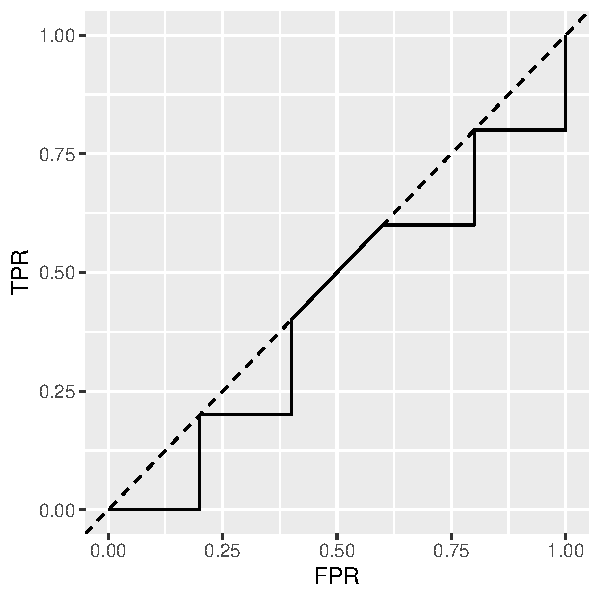
\includegraphics[width=\maxwidth]{figure/unnamed-chunk-25-1} 

}


\end{knitrout}

We see that the resulting ROC lies below the line from the origin with a slope of 1, which represents
a random classifier, i.e., the scoring algorithm performs worse than a random classifier.
If this happens while evaluating the training data, the labels of the scoring algorithm should be inverted.

  \item[d)] 
  We can compute the AUC (\textit{area under the curve}) by looking at the ROC, s.t.
  $$
  AUC = 0.5 - 4 \cdot (0.2 \cdot 0.2 \cdot 0.5) = 0.42.
  $$

\end{enumerate}
}

% ------------------------------------------------------------------------------
% PAST EXAMS
% ------------------------------------------------------------------------------

\dlz
\exexams
\lz

% ------------------------------------------------------------------------------

\aufgabeexam{WS2020/21}{main}{3}{

Consider a binary classification algorithm that yielded the following results 
on 8 observations. The table shows  true classes and  predicted probabilities
for class 1:

\begin{tabular}{ | c | c | c | }
  \hline
  ID & True Class & Prediction  \\ \hline
  1 & 1 & 0.50  \\
  2 & 0 & 0.01  \\
  3 & 0 & 0.90  \\
  4 & 0 & 0.55  \\
  5 & 1 & 0.10  \\
  6 & 1 & 0.72  \\
  7 & 1 & 0.70  \\
  8 & 1 & 0.99  \\
  \hline
\end{tabular}

\begin{enumerate}
  \item Draw the ROC curve of the classifier manually. Explain every step 
  thoroughly, and make sure to annotate the axes of your plot.
  \item Calculate the AUC of the classifier. Explain every step of your 
  computation thoroughly.
  \item Calculate the partial AUC for FPR $\leq 1/3$. Explain every step of your 
  computation thoroughly.
  \item Create a confusion matrix assuming a threshold of 0.75. Point out which 
  values correspond to true positives (TP), true negatives (TN), false positives 
  (FP), and false negatives (FN).
  \item Compute sensitivity, specificity, negative predictive value, positive 
  predictive value, accuracy and F1-score. State the respective formulas first.
  \item In the following plot, you see the ROC curves of two different 
  classifiers with similar AUC's. Describe a practical situation where you would 
  prefer classifier 1 over classifier 2 and explain why. (Note: The data in this 
  question is not related to the data of the above questions.)

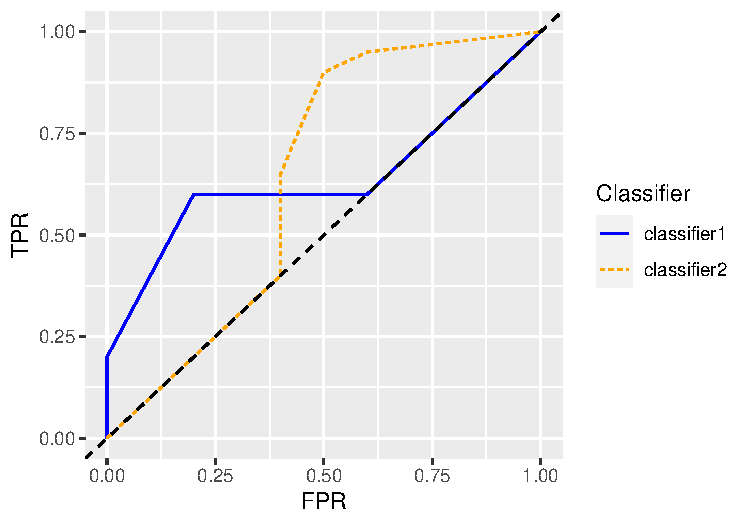
\includegraphics[width=\maxwidth]{figure/unnamed-chunk-11-1} 

\end{enumerate}

}

\dlz
\loesung{

\begin{enumerate}

  \item Scores: \\
\begin{knitrout}
\definecolor{shadecolor}{rgb}{0.969, 0.969, 0.969}\color{fgcolor}
\begin{tabular}{l|r|r}
\hline
  & true\_labels & scores\\
\hline
8 & 1 & 0.99\\
\hline
3 & 0 & 0.90\\
\hline
6 & 1 & 0.72\\
\hline
7 & 1 & 0.70\\
\hline
4 & 0 & 0.55\\
\hline
1 & 1 & 0.50\\
\hline
5 & 1 & 0.10\\
\hline
2 & 0 & 0.01\\
\hline
\end{tabular}

\end{knitrout}
  Here we see that $\frac{1}{n_+} = \frac{1}{5} = 0.2$ and $\frac{1}{n_-} = 
  \frac{1}{3}$. Now we follow the algorithm as described in the lecture slides:
  \begin{itemize}
    \item Set  $\tau = 1$, so we start in $(0,0)$; we predict everything as 1.
    \item Set  $\tau = 0.95$ yields TPR $0 + \frac{1}{n_+} = 0.2$ and FPR  0. 
    (Obs. 8 is '1')
    \item Set  $\tau = 0.8$ yields TPR $0.2$ and FPR  $0 + \frac{1}{n_-} = 1/3$. 
    (Obs. 3 is '0')
    \item Set  $\tau = 0.71$ yields TPR $0.2 + \frac{1}{n_+} = 0.4$ and FPR  
    $1/3$. (Obs. 6 is '1')
    \item Set  $\tau = 0.6$ yields TPR $0.4 + \frac{1}{n_+} = 0.6$ and FPR  
    $1/3$. (Obs. 7 is '1')
    \item Set  $\tau = 0.52$ yields TPR $0.6$ and FPR  $1/3 + \frac{1}{n_-} = 
    2/3$. (Obs. 4 is '0')
    \item Set  $\tau = 0.3$ yields TPR $0.6+ \frac{1}{n_+} = 0.8$ and FPR  
    $2/3$. (Obs. 1 is '1')
    \item Set  $\tau = 0.05$ yields TPR $0.8 + \frac{1}{n_+} = 1$ and FPR  
    $2/3$. (Obs. 5 is '1')
    \item Set  $\tau = 0$ yields TPR $1$ and FPR  $2/3 + \frac{1}{n_-} = 1$. 
    (Obs. 2 is '0')
  \end{itemize}
  Therefore we get the polygonal path consisting of the ordered list of vertices 
  \[(0,0), (0,0.2), (1/3,0.2), (1/3,0.4), (1/3,0.6), (2/3,0.6), (2/3,0.8), 
  (2/3, 1), (1, 1).\]
\begin{knitrout}
\definecolor{shadecolor}{rgb}{0.969, 0.969, 0.969}\color{fgcolor}
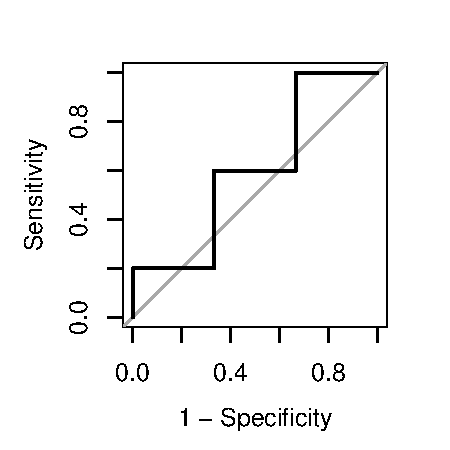
\includegraphics[width=\maxwidth]{figure/unnamed-chunk-13-1} 
\end{knitrout}
  
  \item The AUC is the sum of three rectangles: $0.2 \cdot 1/3 + 0.6 \cdot 1/3 + 
  1\cdot 1/3 = 0.6$
  
  \item The partial AUC is the area under the curve that is left from 
  FPR $= 1/3$, so it is just the first rectangle: $0.2 \cdot 1/3 = 1/15$
  
  \item \phantom{foo}
  \begin{tabular}{ | c | c | c | } \hline
    & Actual Class - 0 & Actual Class - 1  \\
    Prediction - 0 & 2 & 4  \\
    Prediction - 1 & 1 & 1  \\ \hline
  \end{tabular}
  so we get
  \begin{tabular}{ | c | c | c | c | }
    \hline
    FN & FP & TN & TP   \\ \hline
    4 & 1 & 2 & 1 \\ \hline
  \end{tabular}
    
  \item $$\text{Sensitivity} = \frac{\text{TP}}{\text{TP} + \text{FN}} =
  \frac{1}{5} $$
  $$\text{Specificity}  = \frac{\text{TN}}{\text{TN} + \text{FP}} =\frac{2}{3}$$
  $$\text{Negative Predictive Value} = \frac{\text{TN}}{\text{TN} + \text{FN}} =
  \frac{1}{3} $$
  $$\text{Positive Predictive Value} = \frac{\text{TP}}{\text{TP} + \text{FP}} =
  \frac{1}{2} $$
  $$\text{Accuracy} = \frac{\text{TP} + \text{TN}}{\text{TP} + \text{TN} + 
  \text{FP} + \text{FN}} =\frac{3}{8} $$
  $$\text{F1-score} = \frac{2\cdot\text{PPV}\cdot\text{Sensitivity}}{\text{PPV}
  +\text{Sensitivity}} = (0.2) / (0.7) = 2/7  $$
  
  \item Important point is to understand that classifier 1 does better in the
  'high scores'. Or: For some threshold below 0.5 the precision is far better
  for classifier 1 than for classifier 2. For example if you want to output a
  certain number of 'most promising customers' this could be a good idea.

\end{enumerate}
}

%-------------------------------------------------------------------------------

\aufgabeexam{WS2020/21}{main}{6}{

Assume a polynomial regression model with a continuous target variable $y$ and 
a continuous, $p$-dimensional feature vector $\xv$ and polynomials of degree 
$d$, i.e., \\ $\fxi = \sum_{j=1}^p \sum_{k=0}^d \theta_{j,k} (\xi_j)^k$ and 
$\yi = \fxi + \epsi$ where the $\epsi$ are iid with $\var(\epsi)=\sigma^2 \ 
\forall i\in \{1, \dots, n\}$. 

\begin{enumerate}
  \item For each of the following situations, indicate whether we would 
  generally expect the performance of a flexible polynomial learner (high $d$) 
  to be better or worse than an inflexible polynomial learner (low $d$). 
  Justify your answer.
  \begin{enumerate}
    \item[(i)] The sample size $n$ is extremely large, and the number of 
    features $p$ is small.
    \item[(ii)] The number of features $p$ is extremely large, and the number of 
    observations $n$ is small.
    \item[(iii)] The true relationship between the features and the response is 
    highly non-linear.
    \item[(iv)] The variance of the error terms, $\sigma^2$, is extremely high.
  \end{enumerate}
\end{enumerate}

}

\dlz
\loesung{

\begin{enumerate}
  \item 
  \begin{itemize}
    \item (i): flexible: because it covers a larger Hypothesis space and we 
    have enough data
    \item (ii): inflexible: to prevent overfitting
    \item (iii): flexible: because it covers a larger Hypothesis space and we 
    have enough data, an inflexible approach would be too restrictive
    \item (iv): inflexible: to prevent overfitting
  \end{itemize}
\end{enumerate}

}


%-------------------------------------------------------------------------------

\aufgabeexam{WS2020/21}{retry}{3}{

Consider a binary classification algorithm that yielded the following results on 
8 observations. The table shows  true classes and  predicted probabilities for 
class 1:

\begin{tabular}{ | c | c | c | }
  \hline
  ID & True Class & Prediction  \\ \hline
  1 & 1 & 0.30  \\
  2 & 0 & 0.91  \\
  3 & 0 & 0.03  \\
  4 & 0 & 0.55  \\
  5 & 0 & 0.45  \\
  6 & 0 & 0.65  \\
  7 & 1 & 0.71  \\
  8 & 1 & 0.98  \\
  \hline
\end{tabular}

\begin{enumerate}
  \item Draw the ROC curve of the classifier manually. Compute all relevant 
  numbers explicitly, state the respective formulas first, and make sure to 
  annotate the axes of your plot.
  \item Calculate the AUC of the classifier. Explain every step of your 
  computation thoroughly.
  \item Calculate the partial AUC for TPR $\geq 2/3$. Explain every step of your 
  computation thoroughly.
  \item Create a confusion matrix assuming a threshold of 0.7. Point out which 
  values correspond to true positives (TP), true negatives (TN), false positives 
  (FP), and false negatives (FN).
  \item Compute sensitivity, specificity, negative predictive value, positive 
  predictive value, accuracy and F1-score. State the respective formulas first.  
  \item Now look at the following plot. Explain thoroughly why the solid line 
  cannot be the ROC curve of a classifier.

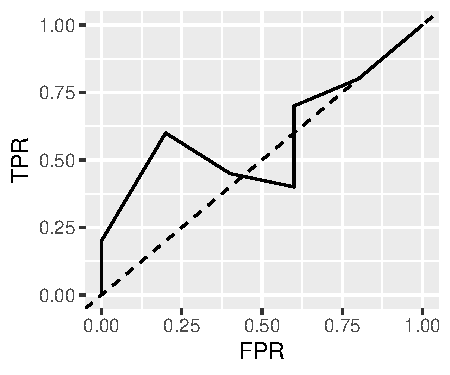
\includegraphics[width=\maxwidth]{figure/unnamed-chunk-14-1} 

  \item Imagine you are working in the marketing department of a large company. 
  Your colleagues are developing a marketing campaign where they will call 
  selected customers by phone in order to advertise a new product. Your company 
  has 1,000,000 customers in the database and the budget of the marketing 
  campaign allows to call 1,000 of these customers. Now it is your job to select 
  the most promising 1,000 customers, i.e., those who will most likely buy the 
  new product after having received the advertising phone call. Luckily, you 
  have a large amount of similar data from older marketing campaigns that are 
  representative for this campaign and can be used to train a supervised 
  classification model with the target variable indicating if the customer did 
  buy the product (1) or not (0). You train a random forest on the 1,000,000 
  observations and get the following cross-validated ROC curve. Assuming a 
  balanced target variable: Do you think this model is fairly good for your 
  purpose? Explain why and describe, how you would proceed from here to provide 
  your colleagues with the 1,000 most promising customers.

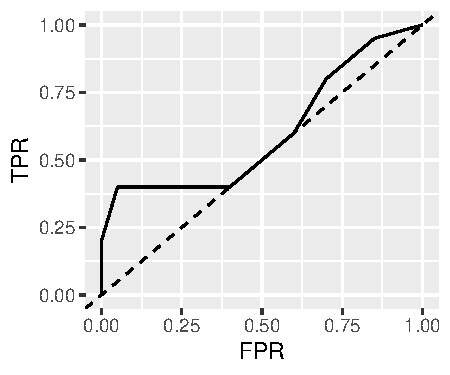
\includegraphics[width=\maxwidth]{figure/unnamed-chunk-15-1} 

\end{enumerate}

}

\dlz
\loesung{

\begin{enumerate}

  \item First we sort the results by score: \\
\begin{knitrout}
\definecolor{shadecolor}{rgb}{0.969, 0.969, 0.969}\color{fgcolor}
\begin{tabular}{l|r|r}
\hline
  & true\_labels & scores\\
\hline
8 & 1 & 0.98\\
\hline
2 & 0 & 0.91\\
\hline
7 & 1 & 0.71\\
\hline
6 & 0 & 0.65\\
\hline
4 & 0 & 0.55\\
\hline
5 & 0 & 0.45\\
\hline
1 & 1 & 0.30\\
\hline
3 & 0 & 0.03\\
\hline
\end{tabular}

\end{knitrout}
  Here we see that $\frac{1}{n_-} = \frac{1}{5} = 0.2$ and $\frac{1}{n_+} = 
  \frac{1}{3}$. Now we follow the algorithm as described in the lecture slides:
  \begin{itemize}
    \item Set  $\tau = 1$, so we start in $(0,0)$; we predict everything as 1.
    \item Set  $\tau = 0.95$ yields TPR $0 + \frac{1}{n_+} = 1/3$ and FPR  0. 
    (Obs. 8 is '1')
    \item Set  $\tau = 0.9$ yields TPR $1/3$ and FPR  $0 + \frac{1}{n_-} = 0.2$. 
    (Obs. 2 is '0')
    \item Set  $\tau = 0.70$ yields TPR $1/3 + \frac{1}{n_+} = 2/3$ and FPR  
    $0.2$. (Obs. 7 is '1')
    \item Set  $\tau = 0.6$ yields TPR $2/3$ and FPR  $0.2 + \frac{1}{n_-} = 
    0.4$. (Obs. 6 is '0')
    \item Set  $\tau = 0.5$ yi´elds TPR $2/3$ and FPR  $0.4 + \frac{1}{n_-} = 
    0.6$. (Obs. 4 is '0')
    \item Set  $\tau = 0.4$ yields TPR $2/3$ and FPR  $0.6 + \frac{1}{n_-} = 
    0.8$. (Obs. 5 is '0')
    \item Set  $\tau = 0.1$ yields TPR $2/3 + \frac{1}{n_+} = 1$ and FPR  $0.8$. 
    (Obs. 1 is '1')
    \item Set  $\tau = 0$ yields TPR $1$ and FPR  $0.8 + \frac{1}{n_-} = 1$. 
    (Obs. 3 is '0')
  \end{itemize}
\begin{knitrout}
\definecolor{shadecolor}{rgb}{0.969, 0.969, 0.969}\color{fgcolor}
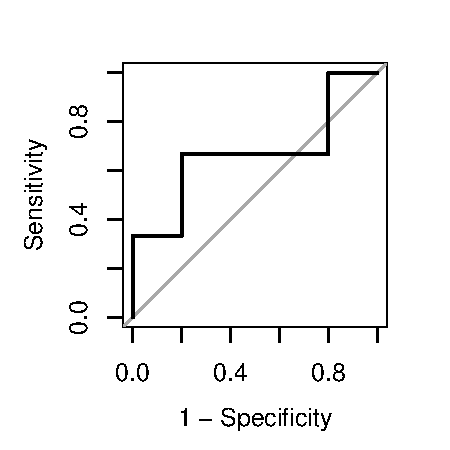
\includegraphics[width=\maxwidth]{figure/unnamed-chunk-17-1} 
\end{knitrout}

  \item The AUC is the sum of three rectangles: 
  $0.2 \cdot 1/3 + 0.6 \cdot 2/3 + 1\cdot 0.2 = 2/3$
  
  \item The partial AUC is the area under the curve that is above TPR $= 2/3$, 
  so it is just the small rectangle in the upper right corner: 
  $0.2 \cdot 1/3 = 1/15$ 
  
  \item   
  \begin{tabular}{ | c | c | c | } \hline
     & Actual Class - 0 & Actual Class - 1  \\
    Prediction - 0 & 4 & 1  \\
    Prediction - 1 & 1 & 2  \\ \hline
  \end{tabular}
  so we get
  \begin{tabular}{ | c | c | c | c | } \hline
    FN & FP & TN & TP   \\ \hline
    1 & 1 & 4 & 2 \\ \hline
  \end{tabular}
  
  \item   
  $$\text{Sensitivity} = \frac{\text{TP}}{\text{TP} + \text{FN}} =\frac{2}{3}$$
  $$\text{Specificity}  = \frac{\text{TN}}{\text{TN} + \text{FP}} =\frac{4}{5}$$
  $$\text{Negative Predictive Value} = \frac{\text{TN}}{\text{TN} + \text{FN}} 
  =\frac{4}{5} $$
  $$\text{Positive Predictive Value} = \frac{\text{TP}}{\text{TP} + \text{FP}} 
  =\frac{2}{3} $$
  $$\text{Accuracy} = \frac{\text{TP} + \text{TN}}{\text{TP} + \text{TN} + 
  \text{FP} + \text{FN}} =\frac{6}{8} $$
  $$\text{F1-score} = \frac{2\cdot\text{PPV}\cdot\text{Sensitivity}}{\text{PPV}
  +\text{Sensitivity}} = (8/ 9) / (4/3) = 2/3  $$
  
  \item TPR and FPR are both metrics that increase monotonically as the 
  threshold $c$ traverses from 1 to 0. The plot shows two instances of 
  diminishing TPR, which would mean that, at the corresponding threshold, an 
  observation that had previously been correctly classified as positive was not 
  detected anymore. This is not possible with a binarization threshold.
  
  \item Yes. I would order the customers wrt the scores, then roughly the first 
  200,000 customers would be true positives (since the ROC is based on 1,000,000 
  customers and true class is balanced) and I would just select the top 1,000 
  customers. It doesn't matter that the classifiers gets bad later.
  
\end{enumerate}

}

% ------------------------------------------------------------------------------
% INSPO
% ------------------------------------------------------------------------------

\dlz
\exinspo
\end{document}
